\documentclass[a4paper,14pt]{extarticle}

% кодировка
\usepackage[utf8]{inputenc}
\usepackage[T2A]{fontenc}

% поля
\usepackage[left=30mm,right=15mm,top=20mm,bottom=20mm]{geometry}

% переносы слов
\usepackage[english,main=russian]{babel}

% шрифт Таймс
\usepackage{tempora}
%\usepackage{newtxmath}
%
% межстрочный интервал
\usepackage[onehalfspacing]{setspace}

% отступ первой строки
\usepackage{indentfirst}
\setlength{\parindent}{1.25cm}

% скрытый структурный элемент
\newcommand{\hidedstructel}[1]{%
    \clearpage
    \section*{#1}%
}

% структурный элемент
\newcommand{\structel}[1]{%
    \hidedstructel{#1}
    \addcontentsline{toc}{section}{#1}%
}

% счетчик приложений
\usepackage{totcount}
\newtotcounter{annexcount}

% приложение
\renewcommand{\thesection}{\Asbuk{section}}
\newcommand{\annex}[1]{%
    \stepcounter{annexcount}%
    \clearpage
    \setcounter{figure}{0}  % сбросить нумерацию внутри раздела
    \setcounter{table}{0}%
    \setcounter{listing}{0}%
    \renewcommand{\thetable}{\thesection.\arabic{table}}
    \renewcommand{\thefigure}{\thesection.\arabic{figure}}
    \renewcommand{\thelisting}{\thesection.\arabic{listing}}
    \section{#1}%
}

% оформление структурного элемента и приложения
\usepackage{titlesec}
\titleformat{\section}
    [display]                   % форма
    {\filcenter\bfseries}       % формат полностью
    {ПРИЛОЖЕНИЕ \thesection}    % метка
    {}                          % отступ от метки
    {}                          % код перед телом

% раздел
\newcommand{\sect}[1]{%
    \clearpage
    \setcounter{figure}{0}  % сбросить нумерацию внутри раздела
    \setcounter{table}{0}
    \setcounter{listing}{0}
    \subsection{#1}
    \renewcommand{\theparagraph}{\thesubsection.\arabic{paragraph}}%
}
\titleformat{\subsection}{\filright\bfseries}{}{}{\thesubsection\hspace{1em}}
\titlespacing*{\subsection}
    {\parindent}    % отступ слева
    {1.5em}              % сверху
    {1.5em}              % снизу
\renewcommand{\thesubsection}{\arabic{subsection}}

% подраздел
\usepackage{placeins}
\newcommand{\subsect}[1]{%
    \FloatBarrier
    \subsubsection{#1}
    \renewcommand{\theparagraph}{\thesubsubsection.\arabic{paragraph}}
}
\titleformat{\subsubsection}{\filright\bfseries}{}{}{\thesubsubsection\hspace{1em}}
\titlespacing*{\subsubsection}
    {\parindent}
    {1.5em}
    {1.5em}

% пункт
\newcommand{\parag}{
    \paragraph{}
}
\titleformat{\paragraph}[runin]{}{\theparagraph}{1em}{ }  % для отступа
\titlespacing*{\paragraph}{\parindent}{}{}

% подпункт
\newcommand{\subparag}{
    \subparagraph{}
}
\titleformat{\subparagraph}[runin]{}{\thesubparagraph}{1em}{ }
\titlespacing*{\subparagraph}{\parindent}{}{}

% содержание
\usepackage{etoc}
\setcounter{tocdepth}{3}

% глубина нумерации разделов
\setcounter{secnumdepth}{5}

% перечисления
\usepackage{enumitem}
\setlist{
    topsep=0,                   % отступ сверху и снизу списка
    partopsep=0,                % то же самое
    leftmargin=0,               % отступ слева
    labelsep=0,                 % отступ метки
    align=left,                 % выравнивание метки
    listparindent=\parindent,   % отступ первой строки абзаца
    itemsep=0,                  % отступ между элементами
    parsep=0                    % отступ между абзацами и элементами
}
\setlist[itemize]{
    label=--~,  % в списках тире короткое, в тексте - длинное
    labelwidth=1.2em,
    itemindent=\parindent+\labelwidth
}
\setlist[enumerate]{
    label=\arabic*),
    labelwidth=1.4em,
    itemindent=\parindent+\labelwidth
}

% перечисление с буквенными метками
\AddEnumerateCounter*{\asbuk}{\c@asbuk}{7}
\newlist{asblist}{enumerate}{2}
\setlist[asblist]{
    label=\asbuk*),
    labelwidth=1.4em,
    itemindent=\parindent+\labelwidth
}

% подписи
\usepackage[singlelinecheck=false]{caption}
\DeclareCaptionLabelSeparator{gost}{~---~}
\captionsetup{labelsep=gost}

% иллюстрация
\newcommand{\fig}[3][1]{
    \begin{figure}[H]
        \centering
        \includegraphics[width=#1\textwidth]{#2}
        \caption{#3}\label{#2}
    \end{figure}
}
\renewcommand{\thefigure}{\thesubsection.\arabic{figure}}
\DeclareCaptionLabelFormat{gostfigure}{Рисунок #2}
\captionsetup[figure]{justification=centering, labelformat=gostfigure, position=bottom}
% font=singlespacing по умолчанию
%skip=-6pt

% листинг
\usepackage[newfloat, cache=false]{minted}
\newcommand{\lst}[2]{
    \begin{listing}[H]
        \centering
        \caption{#2}\label{#1}
        \begin{minipage}[t]{.8\textwidth}
            \inputminted[
                fontsize=\small,
                frame=single,
                breaklines,
                linenos
            ]{text}{#1}
        \end{minipage}
    \end{listing}
}
\renewcommand{\thelisting}{\thesubsection.\arabic{listing}}
\DeclareCaptionLabelFormat{custlisting}{Листинг #2}
\captionsetup[listing]{justification=raggedright, labelformat=custlisting, position=top}

% размер номера строки
\renewcommand{\theFancyVerbLine}{\rmfamily{\small \oldstylenums{\arabic{FancyVerbLine}}}}

% код в документе
\newenvironment{codepiece}[2]
{
    \VerbatimEnvironment
    \begin{listing}[H]
        \centering
        \caption{#2}\label{lst:#1}
        \begin{minipage}[t]{.8\textwidth}
            \begin{minted}[
                fontsize=\small,
                frame=single,
                breaklines,
                linenos
            ]{text}
}{
            \end{minted}
        \end{minipage}
    \end{listing}
}

% таблица
\newenvironment{tbl}[3]
{
    \begin{table}[H]
        \small
        \centering
        \caption{#2}\label{tbl:#1}
        \begin{tabular}{|#3|}
            \hline
}{
            \hline
        \end{tabular}
    \end{table}
}
\renewcommand{\thetable}{\thesubsection.\arabic{table}}
\DeclareCaptionLabelFormat{gosttable}{Таблица #2}
\captionsetup[table]{justification=raggedright, labelformat=gosttable, position=top}

\usepackage{tabularx}

% объединение строк
\usepackage{multirow}
\newcommand{\mr}[2]{\multirow[t]{#1}{=}{#2}}

% колонки
\usepackage{array}
\newcolumntype{M}[1]{>{\centering\arraybackslash}m{#1}}
\newcolumntype{N}[1]{>{\raggedright\arraybackslash}p{#1}}

% заголовок таблицы
\usepackage{xparse}
\NewExpandableDocumentCommand\thead{t< t> O{1} m m}{%
    \IfBooleanTF{#1}{%
        \IfBooleanTF{#2}{%
            \multicolumn{#3}{|M{#4}|}{#5}%
        }{%
            \multicolumn{#3}{|M{#4}}{#5}%
        }
    }{%
        \IfBooleanTF{#2}{%
            \multicolumn{#3}{M{#4}|}{#5}%
        }{%
            \multicolumn{#3}{M{#4}}{#5}%
        }%
    }%
}

% код в таблице
\newenvironment{tabcode}[1]
{
    \VerbatimEnvironment
    \begin{minipage}[t]{#1\textwidth}
    \begin{minted}[fontsize=\small, breaklines]{text}
}{
    \end{minted}
    \end{minipage}
}

% длинная таблица
\usepackage{longtable}
\newenvironment{longtbl}[3]
{
    \small
    \begin{longtable}{|#3|}
        \caption{#2}\label{tbl:#1}\\
        \hline
}{
        \hline
    \end{longtable}
}

% математика
\usepackage{mathtools}  % amsmath
\numberwithin{equation}{subsection}

% графики
\usepackage{tikz, pgfplots}
\pgfplotsset{compat=newest}

\usepackage{csquotes}
\usepackage{adjustbox}
\usepackage{float}
\usepackage{url}

% источники
\usepackage[%
    backend=biber,%
    bibstyle=gost-numeric%
]{biblatex}
\addbibresource{bibliography.bib}
\newcommand{\showbib}{%
    \structel{СПИСОК ИСПОЛЬЗОВАННЫХ ИСТОЧНИКОВ}%
    \printbibliography[heading=none]%
}

% отступы в источниках
\defbibenvironment{bibliography}
    {\list
        {}
        {\setlength{\leftmargin}{0}%
         \setlength{\itemindent}{\parindent}%
         \setlength{\itemsep}{0}%
         \setlength{\parsep}{0}}}
    {\endlist}
    {\item
     \printtext[labelnumberwidth]{%
        \printfield{labelprefix}%
        \printfield{labelnumber}%
     }%
     \hspace{0.5em}}

% метка без точки
\DeclareFieldFormat{labelnumberwidth}{#1}

% номер последней страницы
\usepackage{lastpage}

% счетчик источников
\newtotcounter{bibcount}
\AtEveryBibitem{
    \stepcounter{bibcount}%
}

% счетчики таблиц и рисунков
\usepackage{xassoccnt}
\newtotcounter{tblcount}
\DeclareAssociatedCounters{table}{tblcount}
\newtotcounter{figcount}
\DeclareAssociatedCounters{figure}{figcount}

%% для отладки
%%\usepackage{showframe}
%%\renewcommand\ShowFrameLinethickness{0.25pt}
%%\renewcommand*\ShowFrameColor{\color{red}}
%%\usepackage{graphicx}


\begin{document}

\newcommand{\signplace}{\underline{\hspace{40mm}}}
\newcommand{\dateblank}{%
    <<\underline{\hspace{10mm}}>> \underline{\hspace{30mm}} 2024 г.%
}
\newlength{\twointerv}\setlength{\twointerv}{28.34pt}

\begin{titlepage}
    \singlespacing
    \setlength{\parindent}{0pt}
    \begin{center}
        Министерство науки и высшего образования Российской Федерации\\
        Фереральное государственное бюджетное образовательное учреждение
высшего образования\\
        Российский государственный гидрометеорологический университет\\
        (РГГМУ)\\
        Институт информационных систем и геотехнологий\\
        Направление подготовки: 09.03.03 <<Прикладная информатика>>\\
        Профиль подготовки: <<Прикладные информационные системы\
        и геотехнологии>>

    \end{center}
    \vspace{\oneinterv}
    \begin{center}
    ВЫПУСКНАЯ КВАЛИФИКАЦИОННАЯ РАБОТА\\
    (БАКАЛАВРСКАЯ РАБОТА)
    \end{center}
    \vspace{\oneinterv}
    На тему: <<Разработка приложения интеллектуального ассистента на базе
    технологий глубокого обучения.>>
    \vspace{\twointerv}

    \vfill

    \begin{tabular}{N{70mm}N{80mm}}
        Научный руководитель,\\
        к.т.н Петров Я.А.& \signplace{}\\
        \vspace{5mm}
        Исполнитель студент группы ПИ-Б20-2-2,\\Попов В.Н. & \signplace{}\\
        \vspace{5mm}
        <<К защите допускаю>>,\\
        Заведующий кафедрой,\\
        к.т.н,\\
        Колбина О.Н.\\
        \dateblank{} & \signplace{}\\
    \end{tabular}

    \vfill

    \begin{center}
        Санкт-Петербург 2024 г.
    \end{center}
\end{titlepage}
\setcounter{page}{2}
\pagestyle{}


\begingroup

\parindent 0pt
\newlength{\pagewidth}\setlength{\pagewidth}{1.1em}

\newlength{\sectnum}\setlength{\sectnum}{8.4em}
\newlength{\ssectnum}\setlength{\ssectnum}{1em}
\newlength{\sssectnum}\setlength{\sssectnum}{2em}

\newlength{\sssectindent}\setlength{\sssectindent}{2em}

\newcommand*{\entrybody}{%
    \raggedright%
    \etocname\nobreak%
    \leaders\etoctoclineleaders\hfill%
    \rlap{\makebox[\pagewidth][r]{\etocpage}}%
    \vspace{0.56em}% хак для отступа
}

\etocsetstyle{section}
    {}
    {\leavevmode\etocifnumbered{\leftskip \sectnum}{\leftskip 0}}
    {\normalsize\etocifnumbered%
        {\llap{\makebox[\sectnum][l]{ПРИЛОЖЕНИЕ \etocnumber}}%
            \parbox[t][][t]{\textwidth-\sectnum-\pagewidth}{\entrybody}}%
        {\parbox[t][][t]{\textwidth-\pagewidth}{\entrybody}}\par}
    {}
\etocsetstyle{subsection}
    {}
    {\leavevmode\leftskip \ssectnum}
    {\normalsize\llap{\makebox[\ssectnum][l]{\etocnumber}}%
        \parbox[t][][t]{\textwidth-\ssectnum-\pagewidth}{\entrybody}\par}
    {}
\etocsetstyle{subsubsection}
    {}
    {\leavevmode\setlength{\leftskip}{\sssectnum+\sssectindent}\relax}
    {\normalsize\llap{\makebox[\sssectnum][l]{\etocnumber}}%
        \parbox[t][][t]{\textwidth-\sssectnum-\pagewidth-\sssectindent}{\entrybody}\par}
    {}

\etocsettocstyle{\hidedstructel{СОДЕРЖАНИЕ}}{}

\tableofcontents

\endgroup


\structel{ВВЕДЕНИЕ}
За последние десятилетия произошел огромный скачок в развитии информационных технологий:
от создания первой электронной вычислительной машины, до сложный генеративных
нейронных сетей (GAN). Сейчас компании проводят множественные исследования
для выявления возможностей таких технологий и необходимости дальнейших
инвестиций в данную отрасль. Одним из представителей GAN стали большие языковые
модели (LLM). В настоящее время лидерами в данной отрасли стали: OpenAI,
которые придумали реализовать интерфейс для взаимодействия с нейройнной сетью 
в виде чата; ПАО Сбербанк, реализовавшие отечественную LLM в условиях изоляции
и ограниченных ресурсов; Meta (признана в РФ экстремистской организацией и 
запрещена), разработавшие малую языковую модель (SLM) LLaMA, ставшая прорывом 
для энтузиастов, у которых нет таких ресурсов для реализации LLM, как у 
больших игроков рынка.

В данной выпускной квалификационной работе 
будет разработана платформа, позволяющая взаимодействовать с ресурсами предприятия,
использующая LLM/SLM для генерации релевантных ответов.

Актуальность данной темы обсуловлена возможностью оптимизации многих процессов, 
увеличении производительности сотрудников, повышении лояльности клиентов.
В контексте высшего учебного заведения (ВУЗ), использование технологий подобного рода
повышает конкуретноспособность ВУЗа, что наряду с предыдущими пунктами является
положительной метрикой.

Объект исследования --- большие языковые модели (LLM).

Предмет исследования --- является применение языковых моделей для бизнеса.

Цель работы --- проектирование и разработка приложения, которое позволяет
взаимодействовать с структурой предприятий посредством интерфейса.

В качестве интерфейса для пользователя была выбрана оболочка в виде чат-бота.
Чат-боты давно вошли в жизнь большинства населения. Это подтверждается 
информацией аналитической компании <<eMarketer>>, согласно которой, чат-ботами
пользуются более 1,4 млрд. человек на планете~\cite{botucount}.

Для выполнения поставленной цели были поставлены следующие задачи:
\begin{itemize}
    \item Выполнить анализ предметной области;
    \item Провести сравнительный анализ информационных систем;
    \item Рассчитать сроки реализации проекта;
    \item Смоделировать схему бизнес-процессов;
    \item Составить описание документов бизнес-процессов;
    \item Сформировать перечень требований к ИС;
    \item Исследовать подходы SWOT\@;
    \item Описать сценарии вариантов использования;
    \item Визуализировать описанные сценарии вариантов использования;
    \item Создать модель диаграммы компонентов;
    \item Создать модель диаграммы развертывания;
    \item Реализовать бизнес-логику ассистента и перенести его в интерфейс бота;
\end{itemize}

В работе будет рассматриваться РГГМУ (далее Университет), но применяться бот
сможет не только в конкретном учебном заведении, а для любых предприятий.

Во время разработки ассистента использовалась методология Agile. Она позволила
работать в удобном темпе и формировать требования во время разработки.

В ходе выполнения практической части выпускной квалификационной
работы были использованы:

Python, LangChain, FAISS, HuggingFace, Transformers, Docker.

\sect{Предпроектный анализ}
\subsect{Анализ предметной области}

Индустрия информационных технологий является одной из наиболее динамичных и 
быстроразвивающихся отраслей, где каждый год появляются новые тенденции и
совершенствуются технологии, которые позволяют улучшить пользовательский опыт 
и приносить большую выгоду бизнесу. Одной из ключевых технологий стала 
технология трансформер, предложенная в статье “Attention is all you need”.

Одной из ключевых особенностей трансформеров является их способность 
обрабатывать большие объемы текста без потери информации для выполнения задач
таких как машинный перевод, обработка естественного языка, когнитивный анализ
текста и генерирование текста. Трансформер состоит из блоков кодировщиков и
декодеров, которые обрабатывают входные данные и генерируют выходные данные.
Большое количество параметров сети позволяет ей улучшить качество работы по 
сравнению с другими моделями. В последнее время наблюдается тренд
на внедрение больших языковых моделей в различные отрасли бизнеса, например
системы автоматических ответов на вопросы, чат-боты, умные помощники. 

Преимуществом таких решений является быстрый поиск информации и выдача её в
удобоваримом виде, когда без использования таких ассистентов на поиск
необходимой информации может потребоваться достаточный промежуток времени.
В данной дипломной работе предлагается разработать информационную 
систему-помощника в виде чат-бота который будет представлять собой полезный
инструмент как для студентов, так и для сотрудников ВУЗа. Основная идея
информационной системы состоит в том, чтобы получить универсальный инструмент
для взаимодействия со всей структурой университета. В рамках чат-бота 
пользователь сможет получить всю необходимую информацию, например информацию о
заселении в общежития, списке необходимых документов для поступления т.п.

В общем и целом, интеграция технологии больших языковых моделей является
актуальной и перспективной темой для дипломной работы, которая позволит изучить
основы построения архитектуры приложения, интеграции технологий в предприятия,
основы работы с нейросетями и машинным обучением, а также тестирования решений,
где нет очевидных метрик для измерения результата.

\subsect{Сравнительный анализ}

На данный момент прямых конкурентов у моего решения нет, но я не отрицаю того,
что в настоящий момент может разрабатываться схожее решение. Из схожих решений
можно отметить следующие решения:

Боты от университетов. Такие решения не имеют возможности масштабирования,
имеют ограниченный пул вопрос/ответ и привязанны к какой-то определенной
платформе.

Virtual Spirits. Эта зарубежная компания специализируется на создании на создании
чат-ботов для различных предприятий. Из преемуществ имеется возможность настройки
внешнего вида бота. 

Сравнение моего приложения и приложений конкурентов приведено на таблице
~\ref{tbl:сравнительный анализ}

\begin{longtbl}{сравнительный анализ}
    {Сравнительный анализ}
    {N{3cm}|N{3cm}|N{3cm}|N{3cm}}
        
    Информационная система & 
    \thead>{3cm}{Удобный сбор информации} & 
    \thead>{3cm}{Возможность неявного поиска} & 
    \thead>{3cm}{Необходимость аутентификации} \\\hline
\endhead
    \mr{3}{Virtual Spirits} & \mr{3}{-} & - & + \\\hline
    \mr{4}{ИС от ВУЗ} & \mr{4}{-} & - & + \\\hline
    \mr{5}{Моя ИС} & \mr{5}{+} & + & - 

\end{longtbl}
Опираясь на проведенный анализ можно подвести некоторый итог:
В итоговой системе не будет системы авторизации, так как мне кажется, что вся
информация должна быть в открытом доступе для всех возможных пользователей ИС.

Под удобным сбором информации подразумевается интутивно понятный процесс 
заполнения базы знаний, который может осуществляться как вручную, так и при 
помощи API, парсинга или других методов получения информации.

Возможность получать информацию не связанную с обучением мне кажется одним из
ключевых преимуществ моей информационной системы: для абитуриентов может быть
важно получить информацию как о возможном расписании, так и о постулении в ВУЦ,
получении БСК или же информации о истории университета.

\subsect{Системный анализ}

Исследование проектируемой ИС проводилось в виде нескольких типов 
анализа: SWOT и ISA\@.

SWOT-анализ — метод стратегического планирования, суть которого заключается в 
выявлении факторов внутренней и внешней среды организации и разделении их на 
четыре категории: Strengths, Weaknesses, Opportunities, Threats.
Сильные и слабые стороны представляют факторы внутренней среды объекта анализа.
В свою очередь возможность и угрозы представляют собой внешнюю среду
объекта анализа.

SWOT анализ находится в таблице~\ref{tbl:swot}

\begin{longtbl}{swot}
    {SWOT анализ}
    {N{2cm}|N{6.5cm}|N{6.5cm}}
        
 & \thead>{6.5cm}{Положительное влияние} & \thead>{6.5cm}{Негативное влияние}  \\\hline
\endhead
\mr{1}{Внутренняя среда} & \mr{1}{--- Актуальность\\--- Простота использования}
& --- Нейросетевые галюцинации  \\
&& --- Необходимость тщательно прорабатывать интеграцию во избежание
проблем с безопасностью \\\hline
\mr{2}{Внешняя среда} & \mr{2}{--- Упрощение навигации по ресурсам ВУЗа\\
--- Получение поддержки от государства }
& --- Регуляции со стороны государства  \\
&& --- Бюрократия с какой-либо стороны
\end{longtbl}

Из положительных аспектов можно выделить простоту конечного использования и
улучшение взаимодействие с предприятием. 

Из отрицательных факторов стоит выделить следующие аспекты: нейросетевые 
галюцинации, проблемы с безопасность и бюрократия. 

Нейросетевые галюцинации --- аномалия, возникающая во время работы нейронной 
сети, влияющая на вывод результат непредсказуемым образом. Например, спросив
о технической оснащенности предприятия нейросеть может начать галлюцинировать и
ответить, что у предприятия есть несколько квантовых суперкомпьютеров, хотя это 
не так. Частично решить эту проблему может грамотный промт-инженеринг, а так
же правильное подмешивание контекста в сам промт.

Проблемы с безопасность можно отнести в ту же категорию. Если занести секретные
данные в базу знаний, то велик шанс утечки информации и попадание её в руки 
злоумышленников. Для обхода этой проблемы нужно внимательно относиться к
информации, которую вы собираетесь хранить в базе знаний и иметь базовые навыки
кибербезопасности.

Бюрократия же не позволит внедрить информационную систему, занести все 
необходимые данные без множества согласований и утверждений со стороны 
вышестоящего руководства.

\subsect{Требования к сервису}\\

Функциональные и нефункциональные требования должны быть определены до начала
реализации ИС, чтобы получить представление о конечном продукте.

Для классификации требований использовалась модель $FURPS$. В следующих 
таблицах были приведены функциональные и нефункциональные требования ИС. Эти 
требования характеризуют поведение ИС. Функциональные требования приведены 
в таблице~\ref{tbl:freq}.

\begin{longtbl}{freq}
    {Функциональные требования}
    {N{2.5cm}|N{14cm}}
        
Номер требования & \thead>{14cm}{Описание} \\\hline
\endfirsthead
\mr{1}{FUN\_1} & При начале общения бот должен представиться и рассказать о
своих возможностях \\\hline

\mr{1}{FUN\_2} & По требованию пользователя бот должен предоставить контактную
информацию вышестоящего руководства\\\hline

\mr{1}{FUN\_3} & По требованию пользователя бот должен предоставить информацию
о расписании\\\hline

\mr{1}{FUN\_4} & По требованию пользователя бот должен предоставить информацию
о списке направлений, на которые можно поступить с определенными предметами\\\hline

\mr{1}{FUN\_5} & По требованию пользователя бот должен предоставить информацию
о университете\\\hline

\mr{1}{FUN\_6} & По требованию пользователя бот должен предоставить актуальную 
информацию о местах проведения практики\\\hline

\mr{1}{FUN\_7} & По требованию пользователя бот должен предоставить информацию 
о проводимых мероприятиях внутри университета\\

\end{longtbl}

В таблице~\ref{tbl:soft} приведены нефункциональные требования, затрагивающие
удобство использования приложения.

\begin{longtbl}{soft}
    {Удобство использования}
    {N{2.5cm}|N{14cm}}
        
Номер требования & \thead>{14cm}{Описание} \\\hline
\endfirsthead

\caption*{Продолжение таблицы \thetable} \\
\hline
Номер требования & \thead>{14cm}{Описание} \\\hline
\endhead

\mr{1}{NFR\_1} & Пользователю предоставляется информация о сервисе \\\hline

\mr{1}{NFR\_2} & Использование сервиса не требует от пользователя какого-либо 
обучения\\\hline

\mr{1}{NFR\_3} & Бот предоставляет как текстовый, так и голосовой интерфейс
для общения\\\hline

\mr{1}{NFR\_4} & По требованию пользователя бот должен предоставить информацию
о списке направлений, на которые можно поступить с определенными предметами\\\hline

\mr{1}{NFR\_5} & Информация, предоставляемая ботом должна быть избыточной\\

\end{longtbl}


В таблице~\ref{tbl:reliability} приведены нефункциональные требования, затрагивающие
надежность сервиса.

\begin{longtbl}{reliability}
    {Надежность сервиса}
    {N{2.5cm}|N{14cm}}
        
Номер требования & \thead>{14cm}{Описание} \\\hline
\endfirsthead

\caption*{Продолжение таблицы \thetable} \\
\hline
Номер требования & \thead>{14cm}{Описание} \\\hline
\endhead

\mr{1}{REL\_1} & Сервиса должен работать 24 часа в сутки 7 дней в неделю, за 
исключением технических перерывов. \\\hline

\mr{1}{REL\_2} & Точность предоставляемой информации зависит от предоставляемых
организацией данных\\

\end{longtbl}

В таблице~\ref{tbl:capacity} приведены нефункциональные требования, затрагивающие
производительность сервиса.

\begin{longtbl}{capacity}
    {Производительность сервиса}
    {N{2.5cm}|N{14cm}}
        
Номер требования & \thead>{14cm}{Описание} \\\hline
\endfirsthead

\caption*{Продолжение таблицы \thetable} \\
\hline
Номер требования & \thead>{14cm}{Описание} \\\hline
\endhead

\mr{1}{PER\_1} & На генерацию ответа у сервиса должно уходить не более
10 секунд\\\hline

\mr{1}{PER\_2} & Для работы боту необходимо: постоянный выход в сеть интернет,
    4ГиБ оперативной памяти. Так же, опционально, чтобы бот был полностью автономен
    необходима видеокарта уровня RTX 3060 и выше для размещения сервиса на SLM
    В противном случае необходимо пользоваться посредником в виде LLM от Сбербанк,
    OpenAI, Mistral и т.п.
\end{longtbl}

В таблице~\ref{tbl:support} приведены нефункциональные требования по поддержке
сервиса.

\begin{longtbl}{support}
    {Поддержка сервиса}
    {N{2.5cm}|N{14cm}}
        
Номер требования & \thead>{14cm}{Описание} \\\hline
\endfirsthead

\caption*{Продолжение таблицы \thetable} \\
\hline
Номер требования & \thead>{14cm}{Описание} \\\hline
\endhead

\mr{1}{SUP\_1} & Установка сервиса осуществляется при помощи сценариев\\\hline

\mr{1}{SUP\_2} & Сервис должен поддерживать как работу с различными типами 
данных, поступающими от предприятия
\end{longtbl}

В таблице~\ref{tbl:safety} приведены нефункциональные требования к безопасности
сервиса.

\begin{longtbl}{safety}
    {Требования к безопасности}
    {N{2.5cm}|N{14cm}}
        
Номер требования & \thead>{14cm}{Описание} \\\hline
\endfirsthead

\caption*{Продолжение таблицы \thetable} \\
\hline
Номер требования & \thead>{14cm}{Описание} \\\hline
\endhead

\mr{1}{SAF\_1} & Сервис должен использовать протокол HTTPS для обмена
информацией\\

\end{longtbl}

Изложенные требования в полной мере описывают работу ИС и позвляют реализовать
корректную работу приложения.

\subsect{Регламентирующие документы}

Для соблюдения законодательства, соответствия требования заказчика,
соответствия стандартам качества и урегулирования многих аспектов работы 
программного обеспечения используются регламентирующие документы: ГОСТ,
пользовательское соглашение, рабочие инструкции и прочие.

Список регламентирующих документов приведен в таблице~\ref{tbl:reg_doc}.

\begin{longtbl}{reg_doc}
    {Регламентирующие документы}
    {N{1cm}|N{9cm}|N{2cm}|N{2cm}}
        
    № & \thead>{9cm}{Наименование документа}&
    \thead>{2cm}{Внутренний документ}&
    \thead>{2cm}{Внешний документ} \\\hline
\endfirsthead
%\caption*{Продолжение таблицы \thetable} \\
%\hline
    \mr{1}{1} & Политика приватности & + & -\\\hline
    \mr{1}{2} & ГОСТ 17657-79 Передача данных. & - & +\\\hline
    \mr{1}{3} & ГОСТ 34.321-96. Информационные технологии. Система стандартов по базам данных. Эталонная модель управления данными & - & +\\\hline
    \mr{1}{4} & ГОСТ Р 51904-2002. Программное обеспечение встроенных систем & - & +\\\hline
    \mr{1}{5} & ГОСТ 19.201-78. Техническое задание. требования к содержанию и оформлению & - & +\\\hline
    \mr{1}{6} & ГОСТ 19.401-78. Текст программы. требования к содержанию и оформлению & - & +\\\hline
    \mr{1}{7} & ГОСТ 34.201-89. Виды, комплектность и обозначение документов при создании автоматизированных систем & - & +\\\hline
    \mr{1}{8} & ГОСТ Р 50779.30-95. Приемочный контроль качества & - & +\\

\end{longtbl}

\subsect{Сроки реализации проекта}\\
Для оценки требуемых ресурсов – времени и денег, разработаем график работ. 
Распишем основные блоки работ – это анализ, проектирование, разработка и
документирование. Таким образом получаем, что на разработку системы потребуется
259 дней, что является довольно быстрым сроком. Для оценки стоимости проекта
возьмем средние зарплаты специалистов и получим что на оплату труда уйдет 1,38
миллиона рублей. График работ представлен на рисунке~\ref{Диаграмма временных затрат.png}
позволяет наглядно оценить длительность и стоимость работ.

\fig[1.0]{Диаграмма временных затрат.png}{Диаграмма затрат}

Так же для наглядности временных затрат была использована <<диаграмма Ганта>>,
позволяющая наглядно отследить каждый этап разработки информационной системы.

\fig[1.0]{Диаграмма Ганта.png}{Диаграмма Ганта}

\sect{Проектирование информационной системы}
\subsect{Концептуальное проектирование}

Для отображения функциональности системы используется диаграмма вариантов
использования, представленная на рисунке~\ref{Диаграмма вариантов использования.drawio.png}.
\fig{Диаграмма вариантов использования.drawio.png}{Диаграмма вариантов использования}

Актор \emph{Пользователь} является обобщением клиентов, которые использует 
систему. Прецедент Приветствует отражает требование FUN\_1. Этот и другие
прецеденты описывают субъект Бот, который на диаграмме выделен рамкой.
Прецедент Рассказывает о возможностях отражает требование FUN\_1.
Актор Образовательная организация является источником данных, которые 
необходимы субъекту. Прецедент \emph{Информация о организации} отражает
функциональные требования: FUN\_2, FUN\_3, FUN\_4, FUN\_5, FUN\_6, FUN\_7, и
используется для логического объединения других прецедентов, для уменьшения 
количества связей на диаграмме и облегчить ее восприятие.

Для понимания перемещения данных внутри приложения была разрабработана схема
перемещения данных, представленная на рисунке
~\ref{Схема перемещения данных.drawio.png}.
\fig[0.3]{Схема перемещения данных.drawio.png}{Схема перемещения данных}

\subsect{Диаграмма компонентов}

Диаграмма компонентов описывает физическое представление системы и является
структурной диаграммой языка унифицированного моделирования. Она определяет
архитектуру разрабатываемой системы, устанавливая зависимости между 
программными компонентами. Кроме того, она предоставляет разработчикам и
архитекторам общую картину архитектуры системы, помогает им лучше понимать ее
структуру и взаимосвязи, а также является полезным инструментом для
коммуникации и документирования архитектурных решений. Разработанная диаграмма
представлена на рисунке~\ref{Диаграмма компонентов.png}.

\fig{Диаграмма компонентов.png}{Диаграмма компонентов}

\subsect{Диаграмма развертывания}

Диаграмма развертывания – это тип UML-диаграммы, которая показывает архитектуру
исполнения системы, включая такие узлы, как аппаратные или программные среды
исполнения, а также промежуточное программное обеспечение, соединяющее их. 
Для каких задач строят диаграммы развертывания:

\begin{enumerate}
    \item Визуализация полной структуры исходного кода
    \item Визуализация узлов системы для определения слабых мест
    \item Обеспечение многократного использования отдельных фрагментов
        программного кода
\end{enumerate}

Диаграмма разрабатываемой информационной системы содержит несколько узлов: 
сервер базы знаний внутри университета, сервер приложения, сервер мессенджера,
на котором базируется бот, конечный аппарат, при помощи которого будет 
производиться взаимодействие с информационной системой.

\fig{Диаграмма развертывания.png}{Диаграмма развертывания}


\subsect{Диаграмма последовательности}

Пайплайн действий таков: пользователь вводит запрос в текстовом формате или 
формате аудио, если сообщение передано в аудиоформате, то происходит 
расшифровка аудиозаписи, после чего полученный текст преобразуется в векторное
представление, далее происходит извлечение подходящих документов методом
ближайших соседей (KNN) из базы знаний, сформированной из документов в базе 
данных.

Далее, наиболее релевантные документы подмешиваются к запросу языковой модели,
после чего языковая модель генерирует ответ, опираясь на полученный контекст.

Последовательность работы приложения приведена в приложении
~\ref{Диаграмма последовательности.png}.

\subsect{Схема базы данных}

В качестве базы данных для хранения изначальных документов для построения 
retirivial использовалась система управления базами данных (СУБД) PostgreSQL\@.
Данное решение обладает рядом преимуществ: высокая производительность при 
работе с большими объемами информации; PostgreSQL является свободным 
программным обеспечением, что позволяет использовать данное ПО для любых 
нужд на бесплатной основе; удобство использования и возможность удобного 
переноса данных из других баз данных. Данные пункты стали ключевыми при выборе 
СУБД для хранения информации. 

Такой выбор СУБД позволяет обеспечить высокую отказоустойчивость. Схема 
хранения данных внутри базы данных указана на рисунке
~\ref{Схема базы данных.png}

\fig[0.5]{Схема базы данных.png}{Схема хранения документов}
В качестве базы данных для хранения представления векторных корпусов из 
документов была выбрана FAISS, так как: её удобно использовать, она использует
меньше памяти, чем другие базы данных для векторов, можно использовать 
вычислительные мощности как процессора, так и видеокарты.

\fig{Схема векторизации документов.png}{Схема векторизации документов}

\subsect{Развертывание приложения}
Планируется, что приложение будет размещаться на мощностях образовательного
учреждения. Для упрощения внедрения было принято решение разработать скрипт
для контейнеризации приложения.

В качестве базового образа был выбран образ с GNU Linux в качестве
операционной системы.
GNU Linux является свободным программым обеспечением, что позволяет
использовать его для любых нужд. На листинге 2.1 отображена конфигурация
Dockerfile.

\begin{codepiece}{in-place code}{Dockerfile}
    FROM python:3.12.3-bullseye
    
    WORKDIR /app
    
    COPY . .
    
    RUN pip install -r --no-cashe-dir req.txt
    
    RUN apt-get update && apt-get install -y nano
    RUN apt-get update && apt-get install -y wget bzip2 libxtst6 libgtk-3-0\
     libx11-xcb-dev libdbus-glib-1-2 libxt6 libpci-dev
    
    CMD ["/bin/bash", "-c", "python main.py"]
\end{codepiece}

Данный файл позволяет создать контейнер, содержащий все необходимые 
необходимые для работы зависимости.

\sect{Разработка системы}
\subsect{Выбор средств разработки}

В качестве языка программирования для разработки системы был выбран Python. 
Выбор связан с набором ПО, необходимым для функционирования сервиса, который
был определен на последнем этапе проектирования. Также Python является
наиболее подходящим языком для работы с искусственным интеллектом, для
него имеется много библиотек, нацеленных на решение конкретных проблем.

В качестве системы управления версиями был выбран Git. В качестве системы 
управления репозиториями был выбран GitHub. С недавнего времени GitHub 
располагает возможностью для создания бесплатных приватных репозиториев ---
никто, кроме авторизовазанных пользователей не будет иметь доступа к вашему
репозиторию.

В качестве системы для написания кода был выбран текстовый редактор NeoVim.
NVim ориентирован на разработку без мыши, что позитивно влияет на скорость 
разработки; можно запустить без графического окружения рабочего стола, что
позволяет использовать данный текстовый редактор как на домашнем персональном
компьютере, так и на сервере, не имеющим графической оболочки. Конфигурация
приведена на листинге Б.1.

Для верстки PDF-документа был использован \LaTeX. С использованием пакетов
данный инструмент позволяет достичь отличных результатов для написания
текстовых документов. Так же данное программное обеспечение является свободным.
\subsect{Структура приложения}

Созданное приложение имеет модульную структуру. Это позволяет распределить
зоны ответственности каждого модуля~\cite{solid}; к тому же это позволяет повысить 
отказоустойчивость конечного приложения. 

Схема файловой структуры показана на листинге 3.1.

\begin{codepiece}{in-place code}{Файловая структура}
|-- Dockerfile
|-- documents
|------about.txt
|------checking.txt
|--  common_questions.txt
|--  deductions_recoveries.txt
|-- embeding_store
|------index.faiss
|------index.pkl
|-- LICENSE
|-- main.py
|-- messages.log
|-- README.md
|-- req.txt
|-- retriveval.py
|-- speech2text.py
|-- tex
|-- text_generator.py
|-- videohandler.py
\end{codepiece}

Файл \emph{Dockerfile} содержит инструкцию для сборки контейнера и последующего
запуска приложения внутри контейнера.

Директория \emph{documents} содержит основные документы в текстовом формате,
предназначенные для дальнейшего перевода их в векторное представление. По мере
развития проекта данный список может меняться.

Директория \emph{embeding\_store} содержит эмбединги документов.

Файл \emph{main.py} запускает основное приложение: запуск retrivial, speech2text,
запуск логирования, а так же телеграмм клиента.

Файл \emph{retrivial.py} несет в себе следующий смысл: перевод корпуса текстов
в векторное представление, извлечение 3х наиболее релевантных документов для
составления контекста, а также обогащение запроса пользователя извлеченной
информацией, для составления ответа.

файл \emph{speech2text.py} представляет собой блок расшифровки в аудио
в текстовый формат, для использования блоком \emph{retrivial.py}, если
это потребуется.

Файл \emph{videohandler.py} представляет собой блок разделения видео- и
звуковых дорожек. Извлеченная звуковая дорожка используется блоком
\emph{speech2text.py}.


\subsect{Расчет надежности программного и аппаратного обеспечения}

Для расчета надежности реализуемого продукта необходимо выявить элементы
системы, которые могут выйти из строя. Для себя я поделил их на 3 категории, и
составил таблицы~\ref{tbl:hardware},~\ref{tbl:software} и~\ref{tbl:stochastic}.
Программная часть, аппаратная часть, независящие от обстоятельств. Данные для
столбца 'Коэффициент надежности' брались из открытых источников.

\begin{longtbl}{hardware}
    {Аппаратная часть}
    {N{2.5cm}|N{3cm}|N{4cm}|N{5cm}}
        
    Номер & \thead>{3cm}{Коэффициент надежности}&
    \thead>{4cm}{Краткое описание}&
    \thead>{5cm}{Что повлечет?} \\\hline
\endfirsthead
%\caption*{Продолжение таблицы \thetable} \\
%\hline
    \mr{1}{1} & 0.99 & Выход из строя жесткого диска (HDD)& Поломка HDD влечет за собой:
потерю данных, простой системы.\\\hline

\mr{1}{2} & 0.99 & Выход из строя процессора (CPU) & Поломка CPU влечет за собой: 
простой системы; если мы используем сервер, то потерю производительности; 
большие траты на замену и обслуживание\\\hline

\mr{1}{3} & 0.87 & Выход из строя графического процессора (GPU) & Выход из строя GPU грозит:
снижением производительности или полным выходом из строя системы, большие
затраты на замену и обслуживание\\\hline

\mr{1}{4} & 0.85 & Выход из строя оперативной памяти & Выход из строя модуля оперативной памяти
не так критичен для системы, модулей памяти несколько и вышел один из них, но
если сломались все плашки оперативной памяти, то система не сможет функционировать.\\\hline

\mr{1}{5} & 0.95 & Выход из блока питания & Выход из строя блока питания сулит
полный выход строя системы
\end{longtbl}


\begin{longtbl}{software}
    {Программная часть}
    {N{2.5cm}|N{3cm}|N{4cm}|N{5cm}}
        
    Номер & \thead>{3cm}{Коэффициент надежности}&
    \thead>{4cm}{Краткое описание}&
    \thead>{5cm}{Что повлечет?} \\\hline
\endfirsthead


\caption*{Продолжение таблицы \thetable} \\
\hline
    Номер & \thead>{3cm}{Коэффициент надежности}&
    \thead>{4cm}{Краткое описание}&
    \thead>{5cm}{Что повлечет?} \\\hline
\endhead

    \mr{1}{1} & 0.93 & Выход из строя модуля, ответственного за перевод звука в текст& 
Выход из строя данного модуля не полечет за собой больших проблем для обычных
пользователей, так как будет доступен обычный текстовый ввод, но для людей с
ограниченными возможностями перестанет быть возможным использование моей 
системы\\\hline

\mr{1}{2} & 0.84 & Выход из строя модуля, ответственного за перевод документов в 
векторное представление & Поломка данного модуля может делиться на две категории:
перестает работать перевод текста в векторное представление и перестает работать
извлечение векторов. В первом случае не все так критично, так как часто обновлять
список актуальных документов не нужно, ведь большая часть информации не меняется.
Если же сломается модуль, ответственный за извлечение векторных представлений,
то система в большей своей части перестанет работать, как задумывалось, но все 
равно будет работать: языковая модель будет выдавать ответы, но не будет иметь
контекста о университете, что негативно повлияет на точность ответа.\\\hline

\mr{1}{3} & 0.77 & Выход из строя модуля клиентского приложения & Выход из строя
клиентского приложения сулит собой: репутационные риски, недоступность приложения
для пользователей

\end{longtbl}


\begin{longtbl}{stochastic}
    {Стохастичные переменные}
    {N{2.5cm}|N{3cm}|N{4cm}|N{5cm}}
        
    Номер & \thead>{3cm}{Коэффициент надежности}&
    \thead>{4cm}{Краткое описание}&
    \thead>{5cm}{Что повлечет?} \\\hline
\endfirsthead
%\caption*{Продолжение таблицы \thetable} \\
%\hline
    \mr{1}{1} & 0.99 -- 0.97 & Массовое отключение интернета & Без подключения к сети
интернет система полностью перестает работать. Это можно будет решить, если 
поднять локальную сеть\\\hline

    \mr{1}{2} & 0.99 -- 0.97 & Отключение электричество & Без электричества система полностью 
перестает работать\\

\end{longtbl}

Расчитывая стохастические переменные я отталкивался от того, что выключить
интернет или электричество на сутки могут от 2 до 10 раз

Так как моя система избыточна: множество модулей позволяют работать другим
модулям при выходе из строя, то я буду считать отказоустойчивость системы по
следующей формуле: $R_{total} = 1 - (1 - R_1)(1 - R_2)\ldots(1 - R_n)$, где 
$R_{total}$ --- общая отказоустойчивости системы, $R_n$ --- отказоустойчивость
компонента системы. 

По расчетам надежность аппаратно-программного комплекса
$\approx 1 - 2.5116e-14$, что я считаю довольно хорошим показателем для
такой системы.

\subsect{Расчет ожидаемого результата экономической эффективности}

Основными затратами для реализации информационной системы являются:

\begin{itemize}
\item Покупка необходимого аппаратного обеспечения для обеспечения работы
    языковой модели
\item В случае, если предприятие не хочет или не может позволить аппаратное 
    обеспечение для развертывания системы на своих мощностях, то оформление 
    подписки у предприятий и аренда мощностей для получения доступа к языковой 
    модели
\item Обслуживание сервера
\end{itemize}

Предполагается несколько концепций для получения прибыли от конечного продукта:
Продажа подписки коммерческим и некомерческим организациям, по предоставлению 
конечного продукта. Для некоммерческих организаций подписка будет стоить от 
5000 рублей в месяц, до 15000 рублей в месяц. В свою очередь для коммерческих
организаций планируется разрабатывать уникальный договор по оформлению подписки
на конечный сервис, для получения максимальной выгоды от сделки.

К подписочной модели получения прибыли так же не исключается возможность продажи
программного обеспечения. В таком случае цена за конечный продукт так же 
определяется уникальным договором. В таком случае конечный потребитель не 
платит за подписку и сам обслуживает всю систему, но имеет над ней полный 
контроль. Со стороны продавца передается документация к программному обеспечению.

Для расчета возврата инвестиций используется следующая формула: 
$ROI = \frac{profit - cost}{cost} \cdot 100\%$
Если считать минимальный доход, то выходят примерно следующие цифры:
$ROI = \frac{60000 - 15000}{15000} \cdot 100\%$,
что равно $300\%$. Но в эти цифры не заложена покупка аппаратного комплекса, 
так как рассматривается ситуация, что я у предприятия есть мощности для 
размещения малой языковой модели.

\subsect{Word2vec}

Для хранения представлений документов в понятном для машины виде используется
подход Word2vec.

Преобразование текстовых корпусов в вектора работает следующим образом:
после передачи на вход программе текста программа создает для каждого слова
вектор, после чего происходит процесс обучения. Во время обучения происходит
попытка предсказать контекст слова, основываясь на его окружении. Например,
если в тексте явно кореллируют слова ``упряжка`` и ``конь``, то эти векторные
представления данных слов будут иметь сходство. Визуализацию данного свойства
можно наблюдать на рисунке~\ref{Word_vector_illustration.jpg}

\fig[0.8]{Word_vector_illustration.jpg}{Взаимосвязь векторов слов}

В конце обучения создается векторное пространство, используемое в дальнейших
этапах работы приложения.

Так как большинство решений не оптимизированы для применения на домашних
персональных компьютерах (ПК) было принято решение переопределить некоторые методы
векторизатора из библиотеки HuggingFace, чтобы улучшить работу на своем ПК.
На листинге 3.2 отображены переопределенные методы.

\begin{codepiece}{in-place code}{Векторизатор}
    class HuggingFaceE5Embeddings(HuggingFaceEmbeddings):
        def embed_query(self, text: str) -> List[float]:
            text = f"query: {text}"
            return super().embed_query(text)
    
        def embed_documents(self, texts: List[str]) -> List[List[float]]:
            texts = [f"passage: {text}" for text in texts]
            return super().embed_documents(texts)
    
        async def aembed_query(self, text: str) -> Coroutine[Any, Any, List[float]]:
            text = f"query: {text}"
            return await super().aembed_query(text)
    
        async def aembed_documents(
            self, texts: List[str]
        ) -> Coroutine[Any, Any, List[List[float]]]:
            texts = [f"passage: {text}" for text in texts]
            return await super().aembed_documents(texts)
\end{codepiece}

\subsect{Поиск подходящих векторов}

Созданное векторное пространство делится на множество кластеров
методом K-средних. Для каждого кластера выставляется центроида для
определения сущности каждого корпуса векторов. Это позволяет не перебирать все
вектора, а проходиться по принадлежности к какой-то сущности. При большом
наборе данных это позволяет быстрее находить необходимый вектор.
На рисунке~\ref{Кластеризация векторов.jpg} схематично отображен алгоритм
кластеризации.

\fig{Кластеризация векторов.jpg}{Визуализация кластеризации векторов}

Наиболее релевантные вектора~\cite{vec} сопоставляются при помощи метода K-ближайших 
соседей. Евклидово расстояние между векторами вычисляется по следующей формуле:\\
\[
    d(x,y)=\sqrt{\sum_{i=1}^{n}{(x_i-y_i)}^2}
\]

Так же для поиска похожих векторов используется косинусное расстояние:

\[
    \cos(\theta) = \frac{A \cdot B}{\| A\| \|B\|} = 
    \frac{\sum_{i=1}^{n}A_i \times B_i}{\sqrt{\sum_{i=1}^{n}(A_i)^2}
    \times \sqrt{\sum_{i=1}^{n}(B_i)^2}}
\]
И хотя данный подход не покрывает все возможные случаи~\cite{leven}, он
является наиболее универсальным.

Визуализацию работы поиска релевантных векторов можно на рисунке
~\ref{Визуализация KNN.png}
\fig[0.769]{Визуализация KNN.png}{Визуализация нахождения релевантных векторов}

\subsect{Генерация текста при помощи поиска и аугментаций}

Для работы системы необходимо подать на вход какой либо текст.
В качестве клиента было выбрано клиентское приложение Telegram, а в качестве
интерфейса для взаимодействия приложения и пользователя TelegramBotAPI, но
в качестве клиента можно использовать и другие платформы: ВК, Яндекс.Алиса,
Одноклассники и прочие. За последнее время боты стали очень популярным
решением~\cite{bots} благодаря удобности и доступности, что позволяет
бизнесу удобно использовать подобные интерфейсы в своих интересах.
Чтобы пользователю было удобно использовать созданное приложение было
принято описать идею приложения, а так же дать ссылку на вызов
функции-помощника. Данный аспект отражает нефункциональные требования
NFR\_1 и NFR\_2.

Для пользователей предусмотренна возможность ввода как текстового сообщения,
так и управления ботом при помощи голоса или видео. Данная возможность
отражает нефункциональное требование NFR\_3.

На листинге 3.3 отображена реализация приветственного сообщения от бота.

\begin{codepiece}{in-place code}{Стартовое сообщение}
    dummy_message = "Ищу ответ..."
    stub = hbold("Бот работает в тестовом режиме – не все ответы могут быть достоверными")
    # Start message
    @dp.message(CommandStart())
    async def command_start_handler(message: Message) -> None:
        """
        This is handler for command `/start`
        """
        await message.answer(
            f"Привет, {hbold('студент')}\n\nПеред тобой бот-асситент ИИСИГТ,\
     подготовленный {hlink('мной', 'https://github.com/yaz0p')} к качестве\
     выпускной квалификационной работы\n\nДанный бот позволяет осуществлять\
     удобную навигацию внутри университета и отвечает на не самые очевидные\
     вопросы. \n\nБот работает на основе большой языковой модели, а\
     информацию о внутренних источниках получает благодаря {hbold('RAG')}.\
     Возможно, я прикреплю сюда git репозиторий с реализацией проекта,\
     чтобы студенты могли изучить работу данного ассистента и/или дополнить\
     его своими идеями.\n\n\
    Пример того, что ты можешь спросить:\n- Адрес какого либо-корпуса\n\
    - Номер приемной комиссии\n- Как поступить в ВУЦ\n- Время приема ректората\
     - Информацию о заселении и медкомиссии\n"
        )
        sleep(2)
        await message.answer(
            f"Для получения инструкции о взаимодействии с\
            ассистентом нажмите /help\n\n\
    {hbold('Внимание, все сообщения логгируются!')}"
        )
\end{codepiece}

После получения сообщения сервером Telegram и передачей сообщения приложению
по протоколу HTTPS, что отражает нефункциональное требование к безопасности
SAF\_1, происходит перевод полученного текста в вектор и сопоставление
полученного вектора с векторами из созданного векторного пространства 
базы знаний. После поиска подходящих векторов происходит обратная трансформация
из векторного пространства в текстовое представление. 

На листинге 3.4 отображен процесс создания контекста и промт для
корректной работы языковой модели.

\begin{codepiece}{in-place code}{Функция для поиска векторов и создания контекста}
    def augment_prompt(self, query: str, _embedings_storage=_embedings_storage):
        results = _embedings_storage(self).similarity_search(query, k=3)
        source_knowledge = "\n".join([x.page_content for x in results])
        augmented_prompt = f"""Используя предоставленный контекст ответь на следующий вопрос.

        Контекст:
        {source_knowledge}

        Вопрос: {query}"""
        return augmented_prompt
\end{codepiece}

Далее обогащенный текстовый запрос подается на вход языковой модели, после чего
проиходит генерация текстовых токенов декодером~\cite{a}. На листинге 3.5
отображен модуль, ответственный за генерацию текста.

\begin{codepiece}{in-place code}{Функция для генерации ответа на заданный вопрос}
        def answer(self, message: Message) -> None:
            prompt = PromptTemplate(
                template="Ответь на поставленный вопрос: {subject}",
                input_variables=["subject"],
            )
    
            output = self.chat(
                [
                    SystemMessage(
                        content="""Ты профессиональный ассистент Российского
                        государственного гидрометеорологического университета,
                        который помогает студентам и преподавателям решать их
                        проблемы: навигация внутри университета, ответ на общие
                        вопросы, касающиеся РГГМУ. Если контекст большой, то
                        используй его по максимуму, но не теряй сути.
                        При ответе на вопросы общайся в деловом стиле и пиши
                        только по существу. """
                    ),
                    HumanMessage(
                        content=prompt.format(
                            subject=self.
                            augmentation.
                            augment_prompt(message)
                        )
                    ),
                ]
            )
    
            return output.content
\end{codepiece}

\structel{ЗАКЛЮЧЕНИЕ}

В процессе работы были выполнены поставленные задачи, и в результате работы был
создан сервис, соответствующий поставленным требованиям. Был проведен
необходимый анализ и эстимация. Поставленная цель была полностью выполнена.

Созданный бот можно найти по адресу \emph{https://t.me/IISIGT\_bot} или по логину 
\emph{@IISIGT\_bot} внутри клиента Telegram.

\showbib

\annex{Диаграмма последовательности}

\begin{figure}[H]
    \centering
    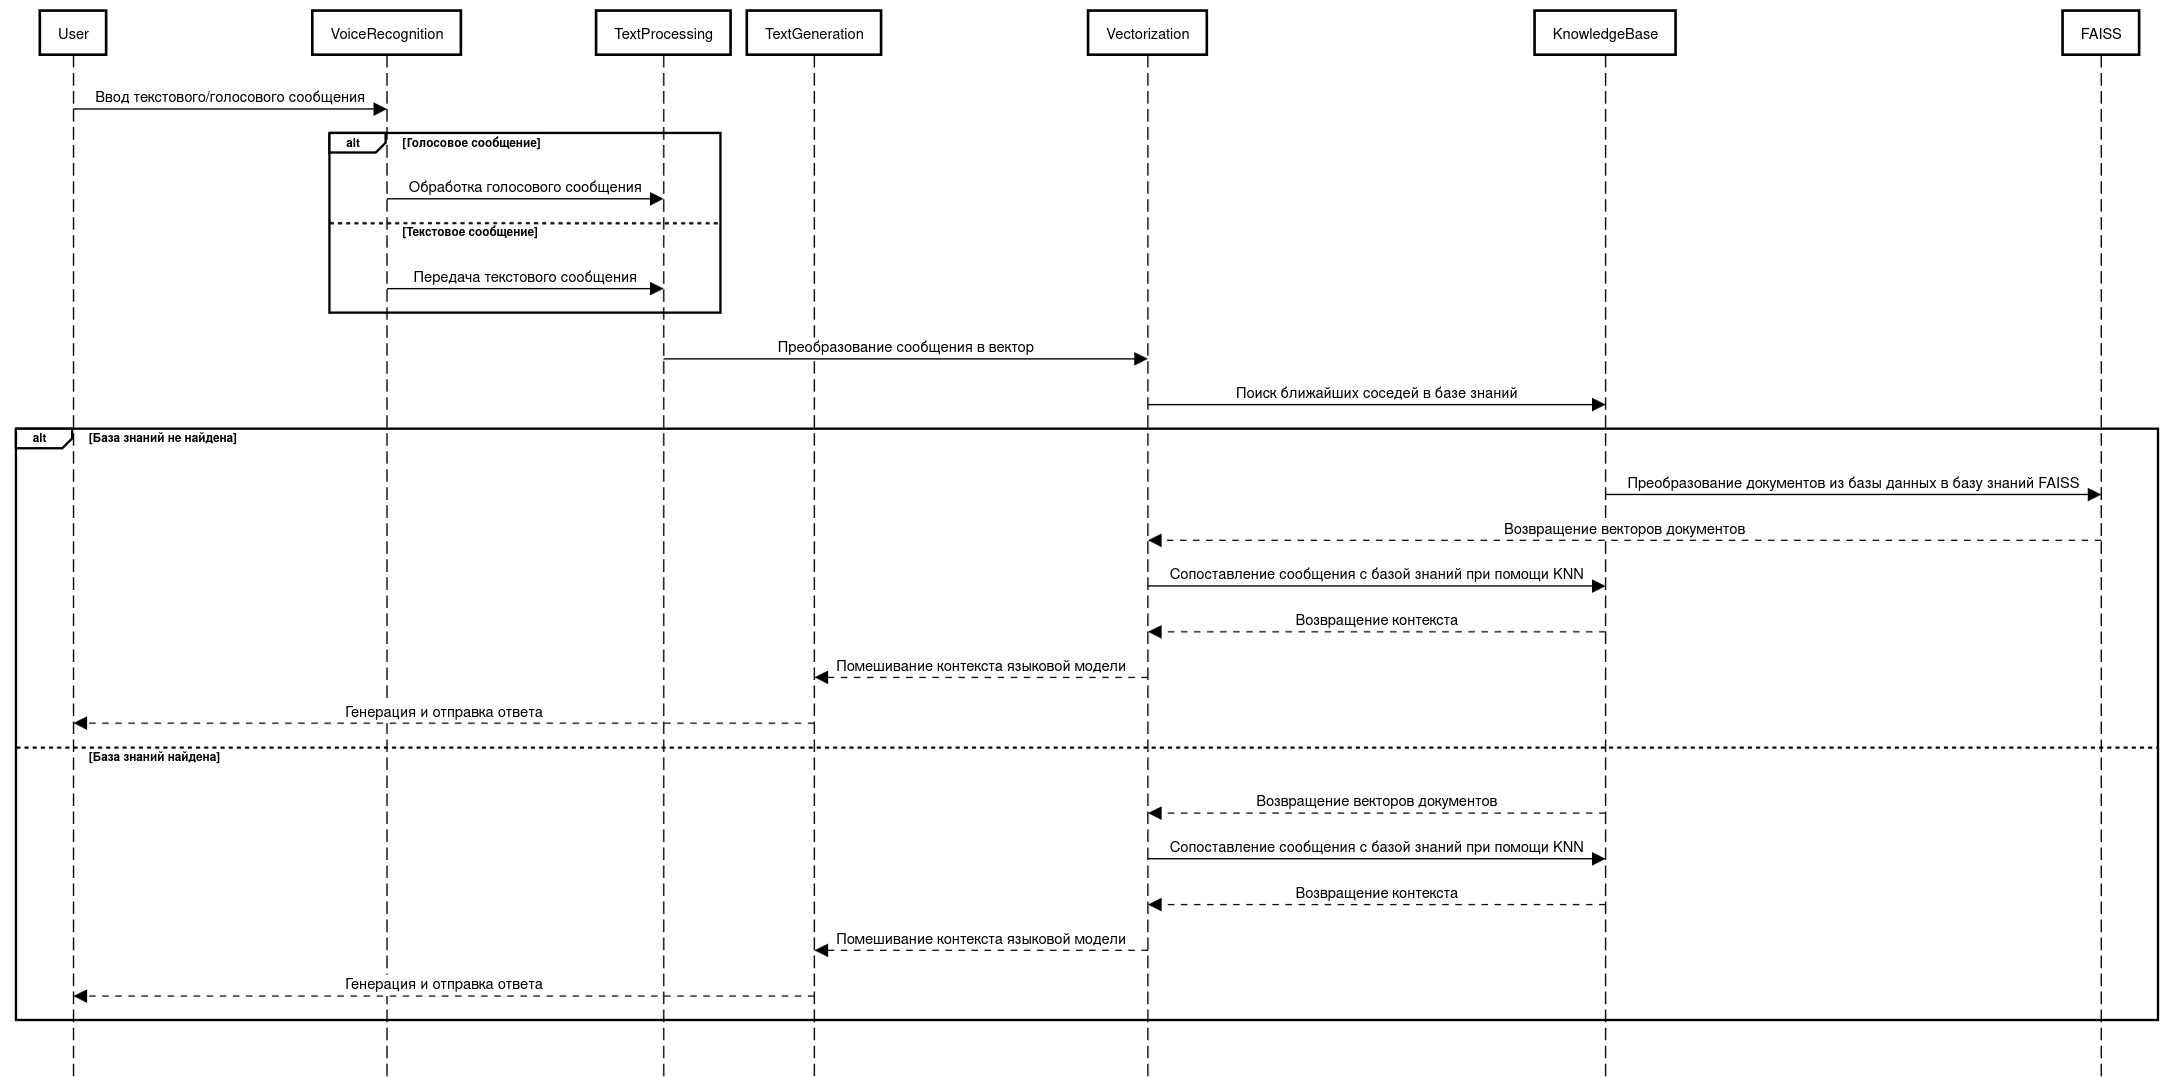
\includegraphics[width=1.2\textwidth, angle=90]{Диаграмма последовательности.png}
    \caption{Диаграмма последовательности}\label{Диаграмма последовательности.png}
\end{figure}

\annex{Конфигурация NeoVim}

\begin{codepiece}{in-place code}{Отрывок конфигурации языкового сервера для работы NeoVim}
local lspconfig = require 'lspconfig'

local capabilities = require('cmp_nvim_lsp').default_capabilities()

lspconfig.pylsp.setup {
  capabilities = capabilities,
  settings = { pylsp = { plugins = require('project.config').pylsp_plugins } },
}
lspconfig.tsserver.setup {
  capabilities = capabilities,
}
lspconfig.ccls.setup {
  capabilities = capabilities,
}
lspconfig.gopls.setup {
  capabilities = capabilities
}

-- `:help vim.diagnostic.*`
vim.keymap.set('n', '<space>e', vim.diagnostic.open_float)
\end{codepiece}

\end{document}
